\section{Исследовательский раздел}

\subsection{Технические характеристики}

Технические характеристики устройства, на котором выполнялись замеры, следующие.

\begin{itemize}[label=---]
	\item Операционная система Windows 10 \cite{oswind} x86\_64.
	\item Память 8 Гб 2400 МГц DDR4.
	\item 1.6 ГГц 4-ядерный процессор Intel Core i5 8265U \cite{intel}.
\end{itemize}

Замеры проводились на ноутбуке, включенном в сеть электропитания. Во время проведения исследований ноутбук был нагружен только встроенными приложениями окружения, а также непосредственно системой выполнения замеров.

\subsection{Подготовка исследования}

Для сравнения производительности разработанного сервера с nginx необходимо установить утилиту для нагрузочного тестирования Apache Benchmark. Данный инструмент позволяет исследовать допустимые границы количества запросов, которое сервер может обработать в секунду.

Также необходимо настроить nginx на отдачу статического контента. Конфигурация nginx представлена в листинге \ref{nginx}.

\begin{lstlisting}[caption={Конфигурация nginx}, label=nginx]
worker_processes  5;
pid        /var/run/nginx.pid;
error_log  /var/log/nginx/error.log info;

events {
\end{lstlisting}

\begin{lstlisting}[title={Продолжение листинга \ref{nginx}}, label=nginx1, firstnumber=6]
	worker_connections  4096; 
}

http {
	charset utf-8;
	
	server { 
		location / {
			root /static;
		}
		
		location /status {
			stub_status;
		}
	}
}
\end{lstlisting}

Для запуска nginx используется Docker. Содержимое используемого файла docker-compose.yml представлено в листинге \ref{compose}.

\begin{lstlisting}[caption={Конфигурация docker-compose.yml}, label=compose]
version: '3.7'
services:  
  nginx:
  image: nginx
  volumes:
    - ./logs:/var/log/nginx
    - ./nginx.conf:/etc/nginx/nginx.conf
    - C:\Users\Pavel\Desktop\parcorpus\static:/static
  ports:
    - "80:80"
    - "443:443"
  restart:
    always
\end{lstlisting}

\subsection{Результаты замеров}

Первый замер проводился для jpg-файла размером 53 Кб. Максимальное число одновременных соединений не превышало 10. На рисунке \ref{jpg-comparison-n} представлена зависимость 50 процентиля p50 (в мс) от числа запросов.

\captionsetup{singlelinecheck = false, justification=centering}
\begin{figure}[H]
	\centering
	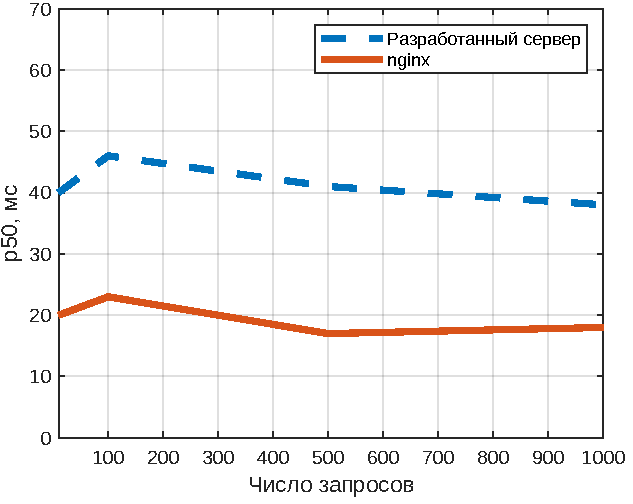
\includegraphics[scale=0.9]{img/jpg.pdf}
	\caption{Зависимость p50 от числа запросов (jpg)}
	\label{jpg-comparison-n}
\end{figure}

Результаты аналогичного замера для pdf-файла размером 2.11 Мб представлены на рисунке \ref{pdf-comparison-n}.

\captionsetup{singlelinecheck = false, justification=centering}
\begin{figure}[H]
	\centering
	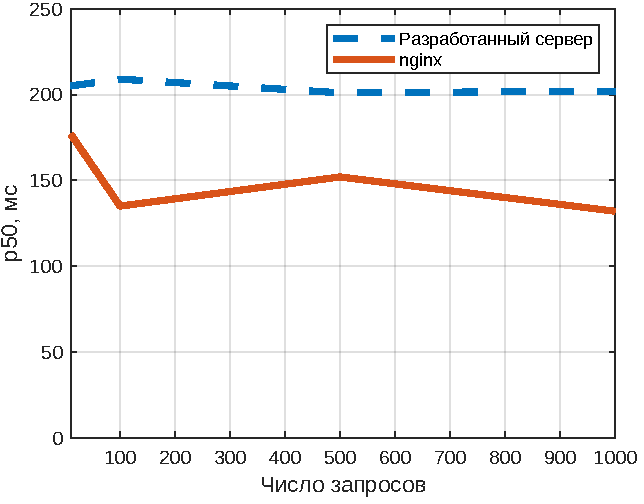
\includegraphics[scale=0.9]{img/pdf.pdf}
	\caption{Зависимость p50 от числа запросов (pdf)}
	\label{pdf-comparison-n}
\end{figure}

Также были произведены замеры при постоянном числе запросов 1000 и изменяющимся максимальным числом конкурентных запросов. На рисунках \ref{jpg-comparison-c} и \ref{pdf-comparison-c} представлена зависимость p50 от числа конкурентных запросов для jpg и pdf файла соответственно.

\begin{figure}[H]
	\centering
	\includegraphics[scale=0.9]{img/jpg-с.pdf}
	\caption{Зависимость p50 от числа конкурентных запросов (jpg)}
	\label{jpg-comparison-c}
\end{figure}

\captionsetup{singlelinecheck = false, justification=centering}
\begin{figure}[H]
	\centering
	\includegraphics[scale=0.9]{img/pdf-с.pdf}
	\caption{Зависимость p50 от числа конкурентных запросов (pdf)}
	\label{pdf-comparison-c}
\end{figure}

\subsection*{Вывод}

В результате проведенных замеров установлено, что разработанный сервер работает медленнее, чем nginx. Время ответа на запросы разработанным сервером в 1.5 -- 2 раза больше, чем время ответа от nginx. Это может быть связано с тем, что nginx -- более оптимизированное программное обеспечение, предназначенное для профессионалов.

Однако нагрузочное тестирование показало, что сервер работает верно: программа корректно обработала все запросы, посылаемые ей в рамках исследования.

\pagebreak